\subsubsection{Beats ($\omega \neq \gamma$)}
\noindent
If $\omega \neq \gamma$, then we can guess that $y_p$ has the form
\begin{equation*}
	y_p = A\cos{(\gamma t)} + B\sin{(\gamma t)}
\end{equation*}
Since we don't have a term involving the 1st derivative, we can be sure that $B = 0$, since an odd number of derivatives is the only way to turn a $\sin$ term into a $\cos$ term. So,
\begin{equation*}
	y_p = A\cos{(\gamma t)}
\end{equation*}
Solving for $A$,
\begin{equation*}
	m\left(A\cos{(\gamma t)}\right)^{\prime\prime} + k\left(A\cos{(\gamma t)}\right) = F_0\cos{(\gamma t)}
\end{equation*}
\begin{equation*}
	-mA\gamma^2\cos{(\gamma t)} + kA\cos{(\gamma t)} = F_0\cos{(\gamma t)}
\end{equation*}
\begin{equation*}
	A\left(k - m\gamma^2\right) = F_0
\end{equation*}
\begin{equation*}
	A = \frac{F_0}{k - m\gamma^2} = \frac{F_0}{m(\omega^2 - \gamma^2)}
\end{equation*}
So, our solution is
\begin{equation*}
	y = \frac{F_0}{m(\omega^2 - \gamma^2)}\cos{(\gamma t)} + C_1\cos{(\omega t)} + C_2\sin{(\omega t)}
\end{equation*}\\

\noindent
Let's look specifically at the IVP where $y(0) = 0$ and $y^\prime(0) = 0$.
\begin{equation*}
	C_1 = \frac{-F_0}{m(\omega^2 - \gamma^2)} \text{ and } C_2 = 0
\end{equation*}
So,
\begin{equation*}
	y = \frac{F_0}{m(\omega^2 - \gamma^2)}\cos{(\gamma t)} - \frac{F_0}{m(\omega^2 - \gamma^2)}\cos{(\omega t)}
\end{equation*}
Using the fact that $\cos{\alpha}-\cos{\beta} = 2\sin{\left(\frac{\alpha - \beta}{2}\right)}\sin{\left(\frac{\alpha + \beta}{2}\right)}$,
\begin{equation*}
	y = \frac{2F_0}{m(\omega^2 - \gamma^2)}\sin{\left(\frac{\gamma - \omega}{2}t\right)}\sin{\left(\frac{\gamma + \omega}{2}t\right)}
\end{equation*}\\

\noindent
When $\gamma \approx \omega$, the $\gamma + \omega$, with a small period, dominates the motion, and the amplitude is slowly guided by the $\gamma - \omega$ term which has a large period. This creates intervals guided by the $\gamma - \omega$ term of higher and lower amplitudes. These are beats.

\begin{center}
	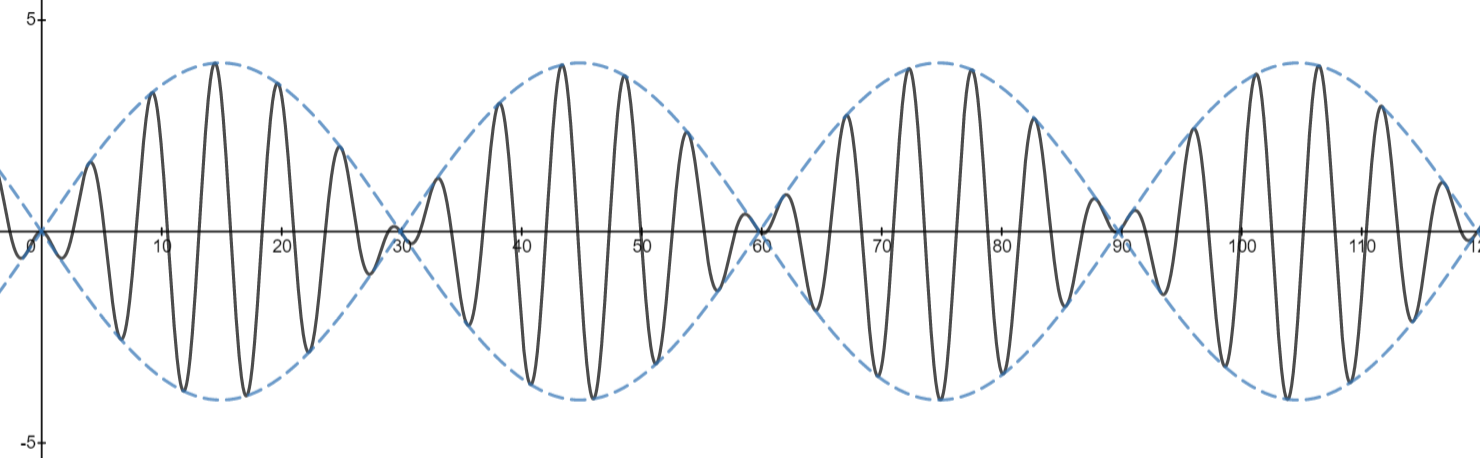
\includegraphics[width=0.75\textwidth]{./higherOrder/forcedVibrs/beats.png}
\end{center}